\section{Étude et cartographie de l'existant}
\label{sec:existant}

\subsection{L'organisation et son écosystème}
La DGSN, rattachée au Ministère de l'Intérieur, est l'autorité de délivrance de la CNIE. Elle s'appuie sur un réseau de centres d'enregistrement des données identitaires (CEDI) répartis sur le territoire, sur deux centres de production (Rabat et Marrakech) qui ont personnalisé respectivement 2,65 et plus d'un million de cartes en 2025 \cite{lavieeco2025bilan}, et sur les services consulaires pour les Marocains résidant à l'étranger. Autour d'elle gravitent l'Agence de Développement du Digital (promotion et support de l'identité numérique), la CNDP (protection des données), la DGSSI (sécurité des systèmes), la Trésorerie Générale pour l'e-timbre, et les fournisseurs de services accrédités à la plateforme Tiers de Confiance National.

\subsection{Les e-services actuels}
Le portail \texttt{cnie.ma} offre quatre fonctions principales \cite{infopratique2026, wadifa2026}~:
\begin{itemize}
  \item la \textbf{pré-demande}, qui recueille le type de demande (première délivrance, renouvellement, duplicata), l'identité en caractères latins et arabes, l'état civil et la filiation, l'adresse de résidence, les coordonnées et un contact d'urgence facultatif destiné à la puce~;
  \item la \textbf{prise de rendez-vous} dans un CEDI, par date et créneau, modifiable ou annulable~;
  \item le \textbf{suivi de la demande} par numéro, avec six statuts (pré-demande, en cours, disponible, remise, dossier incomplet, annulée)~;
  \item des services annexes~: demande de code PIN, prise en charge des cas particuliers (personnes alitées ou handicapées) et information sur les pièces à fournir.
\end{itemize}
Le paiement s'effectue par e-timbre de 75~DH (50~DH avant douze ans), acheté auprès des canaux agréés. La carte est valable dix ans pour les adultes.

À côté de ce portail, la DGSN exploite \texttt{identitenumerique.ma} et l'application «~Mon identité numérique~», qui permettent au porteur d'activer son identité dérivée de la carte, de gérer ses consentements et ses moyens d'authentification, et d'être alerté à chaque usage \cite{dgsn2023tcn}~; ainsi que \texttt{epolice.ma}, qui regroupe depuis fin 2024 des téléservices de police \cite{telquel2024epolice}.

\subsection{Le processus actuel}
La figure~\ref{fig:bpmn-asis} modélise le processus actuel tel que vécu par le citoyen. Trois ruptures de canal le caractérisent~: la pré-demande numérique se termine par l'impression et la signature d'un formulaire papier~; le contrôle des pièces n'intervient qu'au guichet, si bien qu'un dossier incomplet se solde par un nouveau rendez-vous~; enfin, le retrait exige un second déplacement, et l'activation de l'identité numérique relève d'une démarche séparée.

\begin{sidewaysfigure*}
\centering
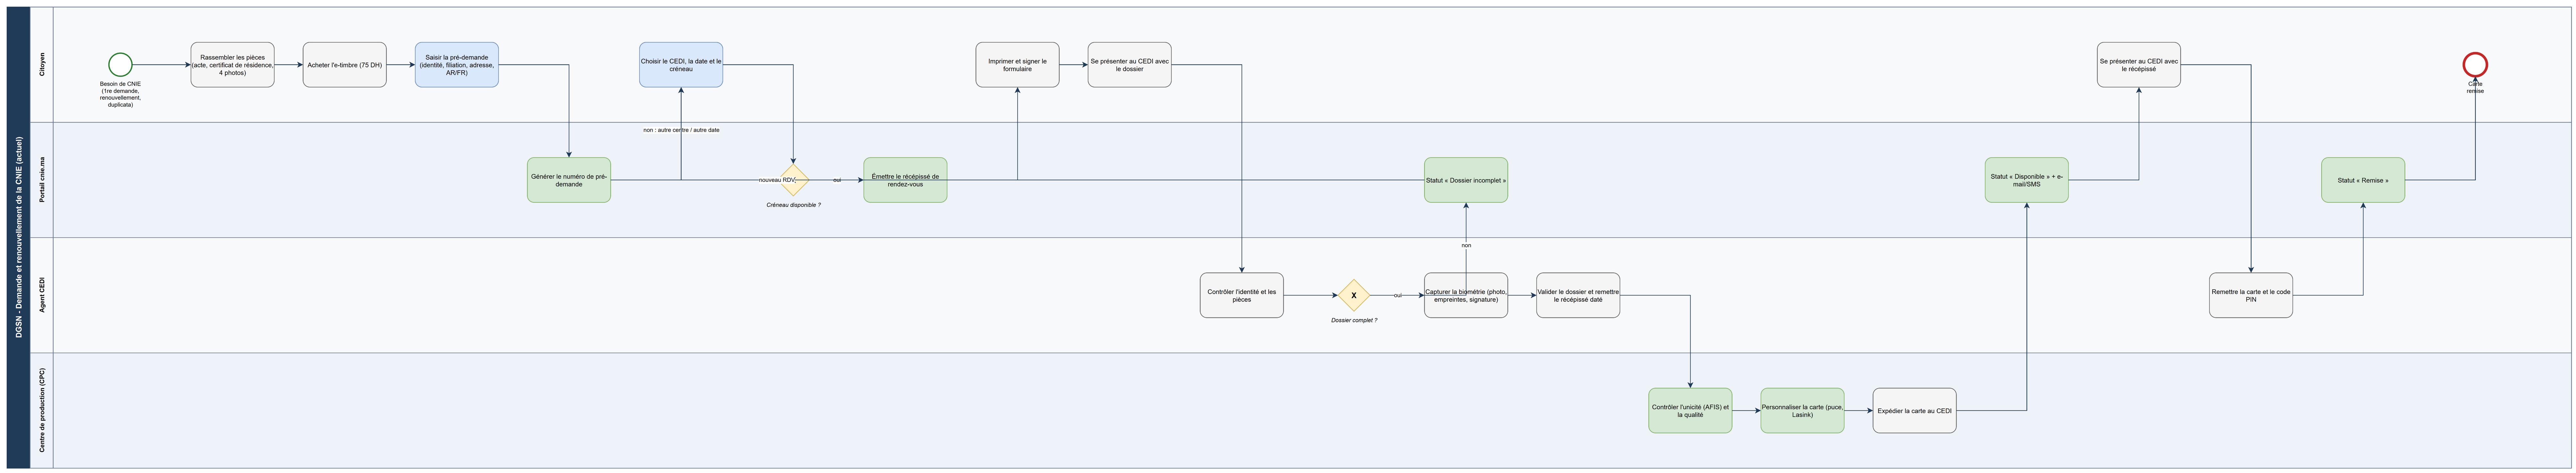
\includegraphics[width=\textwidth]{bpmn/P0_demande_cnie_asis.png}
\caption{Processus P0 actuel (as-is)~: demande et renouvellement de la CNIE. Bleu~: tâches utilisateur sur le portail~; gris~: tâches manuelles~; vert~: tâches automatiques.}
\label{fig:bpmn-asis}
\end{sidewaysfigure*}

\subsection{Cartographies de l'existant}
\paragraph{Fonctionnel} Le SI actuel couvre les fonctions de pré-demande, de rendez-vous, de suivi, d'enrôlement biométrique, de production, de gestion du cycle de vie de la carte (révocation, PIN) et d'identité numérique. Il ne couvre pas, ou seulement manuellement, le contrôle documentaire, l'instruction à distance, la gestion des réclamations, la prévision de charge et le pilotage.
\paragraph{Applicatif} On identifie un portail web, un système de rendez-vous, les postes d'enrôlement des CEDI reliés au référentiel biométrique (AFIS/ABIS), le système de production et de personnalisation, la plateforme Tiers de Confiance National et ses kits hors-ligne, et des échanges ponctuels avec l'e-timbre et les consulats. Les portails sont développés et exploités séparément.
\paragraph{Technique} La plateforme d'identité est décrite par la DGSN comme un système souverain, hébergé et opéré en interne, fondé sur la lecture NFC de la puce, le PIN et la biométrie, et exposé aux partenaires via OpenID Connect \cite{dgsn2023tcn, oidc}.

\subsection{Diagnostic}
\begin{table}[h]
\caption{Synthèse du diagnostic de l'existant}
\label{tab:diag}
\centering
\small
\begin{tabularx}{\columnwidth}{lX}
\toprule
\textbf{Forces} & Couverture nationale quasi complète de la CNIE~2~; rendez-vous en ligne généralisé~; plateforme d'identité numérique souveraine, sans registre central, déjà adoptée par plus de trente partenaires~; capacités de production éprouvées. \\
\midrule
\textbf{Faiblesses} & Contrôle des pièces manuel et tardif~; double saisie (portail puis papier)~; statuts de suivi grossiers, pas de délai annoncé~; renouvellement aussi lourd qu'une première demande malgré une biométrie déjà connue~; canaux et portails en silos. \\
\midrule
\textbf{Opportunités} & Digital Morocco 2030 et loi 55-19~; maturité de l'OCR, de la vision par ordinateur et des modèles de langue~; application mobile d'identité comme futur canal unique~; données historiques de rendez-vous exploitables pour la prévision. \\
\midrule
\textbf{Menaces} & Fraude documentaire et usurpation~; saturation des centres aux pics de renouvellement~; fracture numérique~; exigences réglementaires (CNDP, DGSSI) et risques de biais des modèles biométriques \cite{grother2019frvt}. \\
\bottomrule
\end{tabularx}
\end{table}
